% Options for packages loaded elsewhere
% Options for packages loaded elsewhere
\PassOptionsToPackage{unicode}{hyperref}
\PassOptionsToPackage{hyphens}{url}
%
\documentclass[
  ignorenonframetext,
  english,
]{beamer}
\newif\ifbibliography
\usepackage{pgfpages}
\setbeamertemplate{caption}[numbered]
\setbeamertemplate{caption label separator}{: }
\setbeamercolor{caption name}{fg=normal text.fg}
\beamertemplatenavigationsymbolsempty
% remove section numbering
\setbeamertemplate{part page}{
  \centering
  \begin{beamercolorbox}[sep=16pt,center]{part title}
    \usebeamerfont{part title}\insertpart\par
  \end{beamercolorbox}
}
\setbeamertemplate{section page}{
  \centering
  \begin{beamercolorbox}[sep=12pt,center]{section title}
    \usebeamerfont{section title}\insertsection\par
  \end{beamercolorbox}
}
\setbeamertemplate{subsection page}{
  \centering
  \begin{beamercolorbox}[sep=8pt,center]{subsection title}
    \usebeamerfont{subsection title}\insertsubsection\par
  \end{beamercolorbox}
}
% Prevent slide breaks in the middle of a paragraph
\widowpenalties 1 10000
\raggedbottom
\AtBeginPart{
  \frame{\partpage}
}
\AtBeginSection{
  \ifbibliography
  \else
    \frame{\sectionpage}
  \fi
}
\AtBeginSubsection{
  \frame{\subsectionpage}
}
\usepackage{iftex}
\ifPDFTeX
  \usepackage[T1]{fontenc}
  \usepackage[utf8]{inputenc}
  \usepackage{textcomp} % provide euro and other symbols
\else % if luatex or xetex
  \usepackage{unicode-math} % this also loads fontspec
  \defaultfontfeatures{Scale=MatchLowercase}
  \defaultfontfeatures[\rmfamily]{Ligatures=TeX,Scale=1}
\fi
\usepackage{lmodern}

\ifPDFTeX\else
  % xetex/luatex font selection
\fi
% Use upquote if available, for straight quotes in verbatim environments
\IfFileExists{upquote.sty}{\usepackage{upquote}}{}
\IfFileExists{microtype.sty}{% use microtype if available
  \usepackage[]{microtype}
  \UseMicrotypeSet[protrusion]{basicmath} % disable protrusion for tt fonts
}{}
\makeatletter
\@ifundefined{KOMAClassName}{% if non-KOMA class
  \IfFileExists{parskip.sty}{%
    \usepackage{parskip}
  }{% else
    \setlength{\parindent}{0pt}
    \setlength{\parskip}{6pt plus 2pt minus 1pt}}
}{% if KOMA class
  \KOMAoptions{parskip=half}}
\makeatother


\usepackage{longtable,booktabs,array}
\newcounter{none} % for unnumbered tables
\usepackage{calc} % for calculating minipage widths
\usepackage{caption}
% Make caption package work with longtable
\makeatletter
\def\fnum@table{\tablename~\thetable}
\makeatother
\usepackage{graphicx}
\makeatletter
\newsavebox\pandoc@box
\newcommand*\pandocbounded[1]{% scales image to fit in text height/width
  \sbox\pandoc@box{#1}%
  \Gscale@div\@tempa{\textheight}{\dimexpr\ht\pandoc@box+\dp\pandoc@box\relax}%
  \Gscale@div\@tempb{\linewidth}{\wd\pandoc@box}%
  \ifdim\@tempb\p@<\@tempa\p@\let\@tempa\@tempb\fi% select the smaller of both
  \ifdim\@tempa\p@<\p@\scalebox{\@tempa}{\usebox\pandoc@box}%
  \else\usebox{\pandoc@box}%
  \fi%
}
% Set default figure placement to htbp
\def\fps@figure{htbp}
\makeatother



\ifLuaTeX
\usepackage[bidi=basic,shorthands=off]{babel}
\else
\usepackage[bidi=default,shorthands=off]{babel}
\fi
\ifLuaTeX
  \usepackage{selnolig} % disable illegal ligatures
\fi


\setlength{\emergencystretch}{3em} % prevent overfull lines

\providecommand{\tightlist}{%
  \setlength{\itemsep}{0pt}\setlength{\parskip}{0pt}}



 


\makeatletter
\@ifpackageloaded{caption}{}{\usepackage{caption}}
\AtBeginDocument{%
\ifdefined\contentsname
  \renewcommand*\contentsname{Table of contents}
\else
  \newcommand\contentsname{Table of contents}
\fi
\ifdefined\listfigurename
  \renewcommand*\listfigurename{List of Figures}
\else
  \newcommand\listfigurename{List of Figures}
\fi
\ifdefined\listtablename
  \renewcommand*\listtablename{List of Tables}
\else
  \newcommand\listtablename{List of Tables}
\fi
\ifdefined\figurename
  \renewcommand*\figurename{Figure}
\else
  \newcommand\figurename{Figure}
\fi
\ifdefined\tablename
  \renewcommand*\tablename{Table}
\else
  \newcommand\tablename{Table}
\fi
}
\@ifpackageloaded{float}{}{\usepackage{float}}
\floatstyle{ruled}
\@ifundefined{c@chapter}{\newfloat{codelisting}{h}{lop}}{\newfloat{codelisting}{h}{lop}[chapter]}
\floatname{codelisting}{Listing}
\newcommand*\listoflistings{\listof{codelisting}{List of Listings}}
\makeatother
\makeatletter
\makeatother
\makeatletter
\@ifpackageloaded{caption}{}{\usepackage{caption}}
\@ifpackageloaded{subcaption}{}{\usepackage{subcaption}}
\makeatother

\usepackage{bookmark}
\IfFileExists{xurl.sty}{\usepackage{xurl}}{} % add URL line breaks if available
\urlstyle{same}
\hypersetup{
  pdftitle={ECN 102: Analysis of Economics Data},
  pdfauthor={Remy Beauregard},
  pdflang={en},
  hidelinks,
  pdfcreator={LaTeX via pandoc}}


\title{\texorpdfstring{ECN 102: Analysis of Economics
Data}{ECN 102: Analysis of Economics Data}}
\subtitle{\texorpdfstring{Chapter 10: Multivariate
Regression}{Chapter 10: Multivariate Regression}}
\author{Remy Beauregard}
\date{}

\begin{document}
\frame{\titlepage}


\begin{frame}{Motivation for Multivariate Regression}
\protect\phantomsection\label{motivation-for-multivariate-regression}
Previously, we modeled and conducted inference on the relationship
between two variables, X and Y. However, we are likely to encounter many
scenarios where we think more than one explanatory variable is important
for explaining an outcome variable. In this case, we need to utilize
multivariate regression.
\end{frame}

\begin{frame}{Challenges of Multivariate Regression}
\protect\phantomsection\label{challenges-of-multivariate-regression}
Multivariate regression is a bit more complicated than bivariate:

\begin{enumerate}
[1)]
\item
  We cannot produce a scatterplot in more than 2 (or 3) dimensions,
  meaning we may not easily be able to visualize our series together in
  a single plot.
\item
  We also cannot compute correlation between more than two variables,
  meaning our statistics will be a bit more complicated.
\item
  We may think that some regressors covary with others, meaning we will
  need to work harder to isolate the unique contribution each regressor
  makes to changes in our outcome variable.
\end{enumerate}
\end{frame}

\begin{frame}[fragile]{Pairwise Correlations}
\protect\phantomsection\label{pairwise-correlations}
We may still want to think about correlation between variables in the
multivariate case, but we are restricting to two variables at a time.
Instead, we may compute and display a set of \textbf{pairwise
correlations}: how each variable of interest varies with all other
variables individually. We have seen an example of this in Stata:

\begin{verbatim}
(obs=69)

             |    price      mpg   weight    rep78
-------------+------------------------------------
       price |   1.0000
         mpg |  -0.4559   1.0000
      weight |   0.5478  -0.8055   1.0000
       rep78 |   0.0066   0.4023  -0.4003   1.0000
\end{verbatim}
\end{frame}

\begin{frame}{The Multivariate Regression Model}
\protect\phantomsection\label{the-multivariate-regression-model}
Our multivariate regression model will look quite similar to the
bivariate model but with additional terms:
\[\hat{y}=b_1+b_2x_2+b_3x_3+...+b_kx_k\]

where \(\hat{y}\) is our outcome or \emph{dependent} variable and
\(x_2...x_k\) are our \(k-1\) independent variables or
\emph{regressors}. \(b_2...b_k\) are then the estimated coefficients
associated with each regressor.

Our \(i^{th}\) observation will be given as
\(\hat{y}_i=b_1+b_2x_{2i}+...+b_kx_{ki}\).
\end{frame}

\begin{frame}{Residuals in Multivariate Regression}
\protect\phantomsection\label{residuals-in-multivariate-regression}
Just like bivariate regression, our \emph{residual} is the vertical
distance between our actual and fitted values: \(e_i=y_i-\hat{y}_i\),
which can now be expanded to
\[e_i=y_i-\underbrace{b_1-b_2x_{2i}-b_3x_{3i}-...-b_kx_{ki}}_{\hat{y}_i}\]

However, we need to know how to estimate the \(k\) unknown coefficients
in our regression model, \(b_1,...,b_k\)
\end{frame}

\begin{frame}{Normal Equations (First-Order Conditions)}
\protect\phantomsection\label{normal-equations-first-order-conditions}
Our \(k\) OLS coefficients are found as the solution to \(k\) first
order conditions or \textbf{normal equations} set equal to zero:
\[\sum_{i=1}^nx_{1i}(y_i-b_1-b_2x_{2i}-...-b_kx_{ki})=0\]
\[\sum_{i=1}^nx_{2i}(y_i-b_1-b_2x_{2i}-...-b_kx_{ki})=0\] \[...\]
\[\sum_{i=1}^nx_{ki}(y_i-b_1-b_2x_{2i}-...-b_kx_{ki})=0\]

We obtain these by applying the chain rule to
\(\frac{\partial}{\partial b_j}\sum_i e_i^2\) for \(j=1,...,k\).
\end{frame}

\begin{frame}{Orthogonality}
\protect\phantomsection\label{orthogonality}
Given our definition of our residual as \(e_i=y_i-\hat{y}_i\) and our
normal equations above, we can rewrite these FOCs as
\[\sum_{i=1}^nx_{ji}e_i=0\text{ for }j=1,...,k\] We see that this means
the sum of the products of each regressor and the residual is zero, also
called \textbf{orthgonality}.

Since we know that our constant term means \(x_{1i}=1\) for all \(i\),
we can show that \(\sum_ie_i=0\) for OLS:
\[\sum_{i=1}^nx_{1i}e_i=0\rightarrow\sum_{i=1}^n1e_i=0\rightarrow\sum_{i=1}^ne_i=0\]
\end{frame}

\begin{frame}{Perfect Collinearity}
\protect\phantomsection\label{perfect-collinearity}
An additional constraint on our multivariate regression is that our
regressors are not \textbf{perfectly colinear} with each other (or with
linear combinations of each other). For example, if we had a regressor
\(x_2=3x_3\), we could not include both \(x_2\) and \(x_3\) in our
multivariate regression.

Even if our regressors are not \emph{perfectly} colinear, we may still
be concerned if two or more of our regressors are highly (but not
perfectly) correlated.

Since we are solving \(k\) FOCs to find \(k\) unknown coefficients, we
also need to ensure that our sample size exceeds our number of
regressors: \(n>k\)
\end{frame}

\begin{frame}{Estimating Coefficients: The Formula for \(b_j\)}
\protect\phantomsection\label{estimating-coefficients-the-formula-for-b_j}
Unlike bivariate regression, we cannot easily express a complete formula
for our coefficient estimates.

If we consider \(b_j\) to be the coefficient on the \(j^{th}\) regressor
in a multivariate regression, our coefficient will be equal to the ratio
of the covariance (with our residual) to the variance of \emph{the
residual of a regression of \(x_j\) on all other regressors}:

\[b_j=\frac{\sum_{i=1}^n\tilde{x}_{ji}(y_i-\bar{y})}{\sum_{i=1}^n\tilde{x}_{ji}^2}=\frac{Cov(\tilde{x}_j,y)}{Var(\tilde{x}_j)}\]

where our residual \(\tilde{x}_{ji}=x_{ji}-\hat{x}_{ji}\) and
\(\hat{x}_{ji}\) is the predicted value of \(x_{ji}\) from a regression
of \(x_j\) on all other regressors \(x_{j'\neq j}\).
\end{frame}

\begin{frame}{Implications of the \(b_j\) Formula}
\protect\phantomsection\label{implications-of-the-b_j-formula}
Given our formula, we can see that:

\begin{enumerate}
[1)]
\item
  \(\tilde{x}_{ji}=x_{ji}-\bar{x}_{ji}\) if \(x_j\) is independent of
  all other regressors
\item
  \(\tilde{x}_{ji}=x_{ji}-\bar{x}_{ji}\) if \(x_j\) is our only
  regressor (\emph{bivariate regression})
\item
  \(\tilde{x}_{ji}=0\) if \(x_j\) is perfectly colinear (exactly
  overlaps) with one or more other regressor \(x_{j'\neq j}\) in our
  model
\end{enumerate}

In cases (1) and (2), we see that \(b_j=b_j^{\text{bivariate}}\) when we
plug in \(\tilde{x}_j\).

In case (3), we see that \(\tilde{x}_j=0\) will mean \emph{we cannot
estimate} \(b_2\) as we will have a zero in our denominator.
\end{frame}

\begin{frame}{Overlapping Variation: Diagram}
\protect\phantomsection\label{overlapping-variation-diagram}
Variation of \(x_j\) overlapping with other regressors:

\begin{figure}[H]

\centering{

\pandocbounded{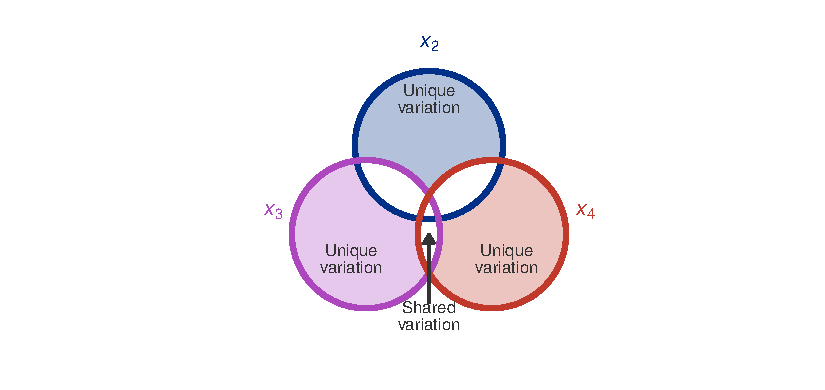
\includegraphics[keepaspectratio,alt={Schematic Venn diagram with three overlapping circles illustrating regressor variation in multivariate OLS. The top circle has a blue border and is labeled x\_2 above it. The bottom-left circle has a purple border and is labeled x\_3 to its left. The bottom-right circle has a red border and is labeled x\_4 to its right. Each circle represents the total variation of one regressor. Only the non-overlapping portion of each circle is shaded, labeled Unique variation outside the circle. The unshaded overlapping regions represent shared variation that cannot be uniquely attributed to any one regressor; an arrow from outside the diagram points to the central overlap region, labeled Shared variation.}]{L10_files/figure-beamer/fig-venn-overlap-1.pdf}}

}

\caption{\label{fig-venn-overlap}Total variation of each regressor (full
circle) and the unique variation used for OLS estimation (shaded
non-overlapping region).}

\end{figure}%
\end{frame}

\begin{frame}{Why Unique Variation Matters}
\protect\phantomsection\label{why-unique-variation-matters}
Why do we need to identify unique variation of \(x_j\), \(\tilde{x}_j\)?

Suppose we want to estimate the associated change in \(y\) when \(x_2\)
changes: this is our coefficient \(b_2\). However, we also know that
\(x_2\) and \(x_3\) are correlated and both appear in our
regression\footnote<\value{beamerpauses}->[frame]{\(y=b_1+b_2x_2+b_3x_3+e\)}.

Now, suppose we observe that:

\begin{itemize}
\item
  \(x_2\) increases
\item
  \(x_3\) increases
\item
  \(y\) increases
\end{itemize}

Did \(y\) increase because \(x_2\) changed? Or did \(y\) increase
because \(x_3\) changed and \(x_2\) changed \emph{because it is
correlated with} \(x_3\)? If variation in \(x_2\) and \(x_3\) (or any
regressors) is allowed to overlap, we cannot identify the \emph{unique}
contribution \(x_2\) makes to changes in \(y\).
\end{frame}

\begin{frame}{Example: Estimating Coefficients in Practice}
\protect\phantomsection\label{example-estimating-coefficients-in-practice}
What would this look like in practice? Suppose we want to estimate
\[\widehat{final}_i=b_1+b_2MT+b_3StataQuiz+b_4HWavg+b_5KCavg\] for your
grade on the final as a function of your other grades in this class. How
would we estimate \(b_3\), the coefficient on \emph{StataQuiz}?

First, we would regress \emph{StataQuiz} scores on all other regressors.
Then, we would find the residuals of this regression. Finally, we would
compute the ratio of the covariance of \(x_3\) residuals with the
residuals from our main regression to the variance of \(x_3\) residuals.
\end{frame}

\begin{frame}{Partial Effect vs.~Total Effect: Definitions}
\protect\phantomsection\label{partial-effect-vs.-total-effect-definitions}
There are two effects from our regressor \(b_j\) we might be interested
in: the \textbf{partial effect} or the \textbf{total effect}

\begin{itemize}
\item
  The \emph{partial effect} is the impact on our outcome variable when
  \(x_j\) changes and \emph{all other regressors are held constant}.
\item
  The \emph{total effect} is the impact on our outcome variable when
  \(x_j\) changes and we allow all other regressors \(x_{j'\neq j}\)
  that may covary with \(x_j\) to change and impact our outcome variable
  through their associated coefficients.
\end{itemize}

It follows that the partial effect will be equal to the total effect if
our regressor \(x_j\) is \emph{independent from all other regressors}
\(x_{j'\neq j}\).
\end{frame}

\begin{frame}{Partial and Total Effects: Formulas}
\protect\phantomsection\label{partial-and-total-effects-formulas}
We express the \textbf{partial effect} as:
\[\frac{\partial\hat{y}}{\partial x_j}=b_j\]

We express the \textbf{total effect} as: \begin{align*}
\frac{d\hat{y}}{d x_j} &= \underbrace{\frac{\partial\hat{y}}{\partial x_j}}_{b_j}\underbrace{\frac{\partial x_j}{\partial x_j}}_1+\sum_{j'\neq j}\underbrace{\frac{\partial\hat{y}}{\partial x_{j'}}}_{b_{j'}}\frac{\partial x_{j'}}{\partial x_j} \\
&= \underbrace{b_j}_{\text{direct effect}}+\underbrace{\sum_{j'\neq j}b_{j'}\frac{\partial x_{j'}}{\partial x_j}}_{\text{indirect effect(s)}}
\end{align*}
\end{frame}

\begin{frame}{Total Effect Equals Bivariate Coefficient}
\protect\phantomsection\label{total-effect-equals-bivariate-coefficient}
With some math, we can also show that the \emph{total effect} of \(x_j\)
in a multivariate regression of y is equal to the \(b_2\) coefficient
from a bivariate regression of y on \(x_j\).

This should make sense: the total effect is the direct effect of \(x_j\)
on y plus any indirect effects through other variables. The sum of these
effects must then be equal to the effect of \(x_j\) on y alone in a
bivariate regression.
\end{frame}

\begin{frame}{Model Fit in Multivariate Regression}
\protect\phantomsection\label{model-fit-in-multivariate-regression}
Luckily, our measures of model fit do not need to change much to
accommodate multivariate regression, since they depend on our residual
(\(e=y-\hat{y}\)):

\begin{itemize}
\item
  RMSE
  \[s_e=\sqrt{\frac{1}{\boldsymbol{n-k}}\sum_{i=1}^n(y_i-\hat{y}_i)^2}\]
\item
  \(R^2\)
  \[\frac{ExpSS}{TSS}=\frac{\sum_{i=1}^n(\hat{y}_i-\bar{y})^2}{\sum_{i=1}^n(y_i-\bar{y})^2}\]
\end{itemize}

Notice: we now have \(n-k\) degrees of freedom in our RMSE denominator,
since we are estimating coefficients on \(k\) regressors (instead of
two) to use in our calculation.
\end{frame}

\begin{frame}{The Problem with \(R^2\)}
\protect\phantomsection\label{the-problem-with-r2}
Unhelpfully, our \(R^2\) will always weakly increase as we add
regressors\footnote<\value{beamerpauses}->[frame]{Since \(\sum e_i^2\)
  will never increase as more regressors are added, R-squared will
  either remain unchanged or increase as more regressors are added.},
but we may face other downsides to endlessly adding regressors to our
model.

We therefore might want to introduce a measure of model fit that:

\begin{enumerate}
[1)]
\item
  Allows us to compare standardized fit between models
\item
  Penalizes models that endlessly add (useless) regressors
\end{enumerate}
\end{frame}

\begin{frame}{Adjusted \(R^2\)}
\protect\phantomsection\label{adjusted-r2}
Thus, we introduce \textbf{adjusted R-squared}:

\[\bar{R}^2=1-\frac{ResSS/(n-k)}{TSS/(n-1)}\in[0,1]\]

This statistic still gives us a standardized measure of model fit but
also \emph{is decreasing in the number of regressors we add} (\(k\)). We
typically prefer to use this statistic for multivariate regressions over
the standard \(R^2\).
\end{frame}

\begin{frame}[fragile,shrink=30]{Multivariate Regression Example}
\protect\phantomsection\label{multivariate-regression-example}
\vspace{3em}

\begin{verbatim}
no; dataset in memory has changed since last saved
r(4);

r(4);
\end{verbatim}

\[\widehat{price}=\underbrace{-1939.87}_{b_1}-\underbrace{52.22}_{b_2}\underbrace{mpg}_{x_2}+\underbrace{2.11}_{b_3}\underbrace{weight}_{x_3}+\underbrace{820.81}_{b_4}\underbrace{rep78}_{x_4}\]
\end{frame}

\section{End of Lecture Material}\label{end-of-lecture-material}

\begin{frame}{Knowledge Check 10}
\protect\phantomsection\label{knowledge-check-10}
\begin{enumerate}
[1)]
\item
  What is the difference between R-squared and adjusted R-squared? Why
  might we prefer the second as a measure of multivariate model fit?
\item
  Why do we have \(n-k\) degrees of freedom in our multivariate RMSE
  instead of \(n-2\)?
\item
  How do we compute the coefficient \(b_j\) in a multivariate regression
  with \(k>2\) regressors (in words)?
\item
  How does the partial effect of \(x_j\) differ from the total effect?
\end{enumerate}
\end{frame}




\end{document}
